\documentclass{article}
\usepackage{graphicx}
\usepackage{csquotes}
\usepackage[firstinits=true]{biblatex}
\usepackage{authblk}
\usepackage{hyperref}
\usepackage{tabularx}
\usepackage{caption}
\usepackage[margin=2cm]{caption}
\captionsetup{justification=centering}



\begin{document}
\title{Malloc}
\author{Fredrik Öberg \\ \href{mailto:fobe@kth.se}{fobe@kth.se}}
\affil{Examiner: Prof. Johan Montelius}
\affil{KTH Royal Institute of Technology, Sweden}
\date{\today}
\maketitle

\begin{abstract}
This paper examines how memory management works in a computer system and touches on topics like how allocation and 
deallocation of physical memory to running processes work and how those practices could be implemented. It also goes through what 
memory overhead is, and how it affects a computers memory. The paper shows that with som added complexity to a memory 
management algorithm a significant increase in memory utilage can be accomplished. This is shown through tests where 
both internal and external memory fragmentation becomes limited as well as a decrease in memory overhead after the implementation
of the added complexity. 

\end{abstract}
\newpage
\tableofcontents
\newpage

\section{Introduction}
This paper is written as a part of the examination of the course ID1206 - Operating Systems; itself part 
of the operations of KTH Royal Institute of Technology. The course provides knowledge of the principles of 
abstractions concerning computer hardware as well as virtualization of resources and timetabling of assignments and
 how those principles can be implemented; mainly as regards to program execution, memory management and 
 persistent storage of data.

 The purpose of this paper is to get a deeper understanding of how an operating system(OS) handles physical 
computer memory allocation and deallocation – a process by which computer programs and services are assigned 
physical memory. This is done by implementing different memory management algorithms and perform testing procedures 
on those algorithms to observe their behavior. The paper also touches on the topic of what can be done 
to increase both the efficiency in terms of memory usage as well as sheer performance. 

\section{Background}\label{background}
A process is an executing instance of a computer program. The process needs computer memory so it can 
perform its intended tasks and asks the computers OS for that amount of memory. This is accomplished by 
calling the OSs memory allocator through an application programming interface(API) the OS provides. 
The memory space is divided into blocks of different size and if the OS finds an available amount of memory 
satisfying the processes request, it marks that block of memory as taken and distributes it to the 
process. When the process is finished using its given memory block it needs to call the allocator once 
again through the OS API but this time telling it to free up the previously used memory block thereby 
making it available to other processes to use.

Each block of memory is assigned its specific header so the OS can keep track of the topology of the memory. The 
headers stores block information such as the size of the block, if it is free or not, how adjacent blocks look 
like etc. all depending on what type of memory manage algorithms are used by the memory allocator. One goal to 
ensure that the memory usage is efficient is to keep the size of the head as small as possible. This is especially 
important in computers with little memory since a large memory overhead used by the block heads then makes up a larger 
percentage of the complete usage of the memory i.e. less memory for the processes to do their work in. How a memory 
allocator manages the allocation and deallocation of 
memory also affects how the memory of a computer system behaves long term. An inefficient allocation algorithm gives 
larger blocks of memory to the processes than they need, thereby creating large internal fragmentation of the memory, 
since a large part of the allocated memory is not used. This situation can be somewhat managed by splitting up large blocks
 into smaller blocks with sizes more fit to the needs of the processes. An inefficient deallocation algorithm will create
 problems as well if it does not handle the freed-up memory in an efficient way. With an allocating algorithm splitting 
 up memory blocks into smaller sizes and a deallocator not merging adjacent free memory blocks a lot of external fragmentations will be 
created since the memory will be split up into smaller and smaller blocks of memory. This will create a lot of
memory overhead since the memory used for block heads will increase which each new block created, and it will also 
create problems for future processes since there might not be blocks large enough for the OS to hand out which satisfies the process requests.

\section{Set Up}\label{setup}
To test out ways to solve the problems raised in the previous part, a basic allocating function was developed using the programming language 
C to check how different allocating algorithm works and what kind of behavior they bring to the memory allocating scheme. 
First was a memory block of 64 kilobytes(kB) allocated from the OS via the Unix system call mmap - a block from this point on called 
the arena - and by that simulating a system with that amount of memory available for the faux processes of the tests to use. 
A list of free blocks was created to keep track of how much memory there was available at a given time. The block headers used to store 
the block information was also created and these headers were in the initial allocating version 24 bytes large. They consisted of 
variables keeping track of the size and status of the current as well as the preceding block in the arena. Two variables were 
also implemented in the headers called next and prev for the free list to use. They enabled for a block who itself was on the list 
to keep track of what free block precedes as well as succeeds it on the free list. The boundaries of the previously created arena 
where set by two of these blocks so that the program could know in what frame the memory blocks could be located. The initial free 
head block thereby consisted initially of 65488 bytes, since 64kB minus 48 bytes for the boundary headers sums up to that amount.


The first allocation algorithm implemented had a way of splitting up free blocks into a size more fit to the current memory 
request in an attempt to limit internal fragmentation. It had on the other hand no way of merging free blocks which the 
next version of the allocation algorithm had. With som added complexity it checked if the blocks before and after it in the arena 
was also free and merged with them if that was the case creating a larger free block with only one header. 
The third and last version of the algorithm a smaller header than the initial implemented, consisting of only eight bytes
worth of variables. The aim was the accomplish a smaller header overhead by adding some complexity to the algorithm without decreasing 
performance in an unreasonable way. This was enabled by removing the next and prev variables if a block was not in the free list. 

The different memory management algorithms was tested by simulating several allocation and deallocation requests of variable sizes. The request were 
between 8 and 1024 bytes in the large header version and 16 and 1024 bytes with the smaller one. The 8 bytes comes from that it is the smallest 
address which can be used if the allocation is to be aligned with the memory of a 64-bit processor. The 16 bytes on the other hand
comes from that the smaller header still needs to occupy a minimum of 24 bytes for the implemented free list to use. 16 bytes also aligns with 
the 64-bit address. Each request size was randomized with the bottom boundary was set at 8 and the top at 1024 bytes. 

The testing involved using 1000 iterations of requests where the process started by allocating memory to 40 requests simulating a startup of 
a system. It thereafter had a 50 percent chance per iteration of making an allocating and/or deallocating request, simulating processes being 
finished as well as new being initated. 

Lastly a performance test was initiated where the performance of the small and the larger header versions was tested and compared to each other 
by allocating 1000 blocks of 16 bytes write to each of those blocks for 10000 iterations. This was done 100 times 
consecutively and the time it took for each one of those 100 write session were timed to see if the memory overhead 
of the different sized blocks had any effect on the computer’s performance.   


\section{Results}\label{results}
The first graph (see Figure \ref{fig:basic}) is the result of the benchmark where no 
merging of contiguous free blocks were initiated. The graph shows a steady increase in the free list size though it seems beginning to 
pan out at the end. The graph also shows as a steady decrease in the average size of the free blocks available. 


\begin{figure}[h!]
    \centering
    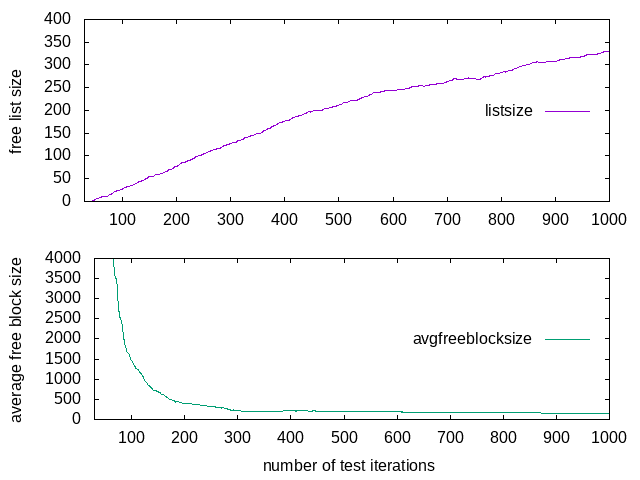
\includegraphics[width=0.8\textwidth]{basic.png}
    \caption{Free list and average free block size development without merging scheme}
    \label{fig:basic}
\end{figure}
\newpage

The second graph (see Figure \ref{fig:merge})shows the result of the test where the merging algorithm had been implemented. It shows an increase 
in the free list size and decrease of the average block size until about 400 request iterations had been made. It then stays at a free 
list size of about 30 and an average free block size of slightly above 1000 bytes. 

The third graph (see Figure \ref{fig:smallMerge})is the result of the test where the smaller block heads had been implemented along with the merging 
scheme. After about 300 request iterations the free list is quite stable at a size of
 slightly above 20 and the average block size is hovering around 2000 bytes. 

The last graph (see Figure \ref{fig:time}) shows the performance test differenc between the different header type merging algorithms. It shows that 
the smaller head version stabilizes at about 6 milli seconds(mS) and the larger version at about 8 mS after an estimated 30 test executions.

\begin{figure}[h!]
    \centering
    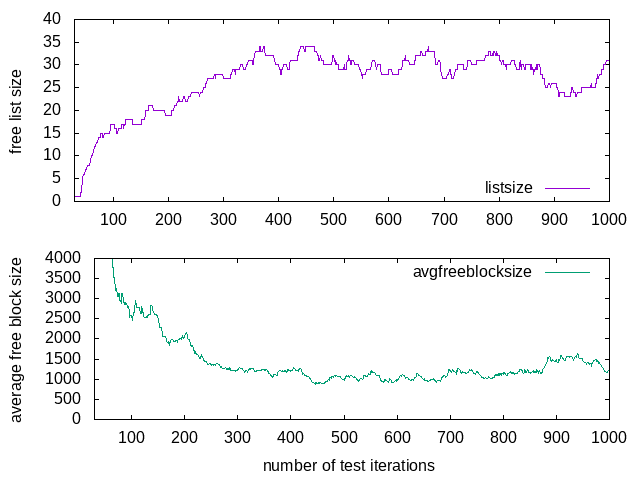
\includegraphics[width=0.8\textwidth]{merge.png}
    \caption{Free list and average free block size development with merging scheme}
    \label{fig:merge}
\end{figure}



\section{Discussion}\label{discussion}

The result visualized in the first graphs clearly show that the size of the free list steadily increases as time
 passes. This is not surprising since for each request of a given size, either a block of exact that size is found in the free list, 
 or a free block of a larger size found and split into two, creating a new block with its own header. Since the algorithm had no way 
 of merging free blocks that means that the free list always increases in size for each deallocated block and as consequence results 
 in free blocks with smaller and smaller sizes.

 \begin{figure}[h!]
    \centering
    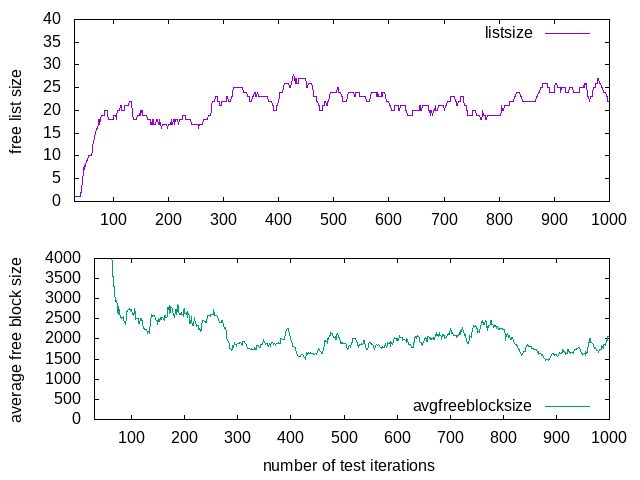
\includegraphics[width=0.8\textwidth]{smallMerge.png}
    \caption{Free list and average free block size development with merging scheme and smaller block head}
    \label{fig:smallMerge}
\end{figure}

 The second graph indicates that the merging algorithm has a free list size which is a sort of a probabilistic equilibrium. 
 When the number of free blocks reaches above this equilibrium it is likely that they will get adjacent free blocks with which it can merge thereby 
decreasing the size free list. That the free list size and the average block size hoovers around
the values they do could be the result of the test implementation and those values could change with another test. However, 
it seems likely that those tests would show a similar behavior as this one, hoovering around a steady value. 

The result of the third test is very similar to the second but shows some increase in the memory usage. The result 
indicates that the free list size equilibrium in this test seem to be at around 20, or at least below what was seen in 
the test with the larger headers. The test also indicates that the average free block size is larger. These observations 
seem reasonable since a smaller memory overhead should result in larger block sizes overall as well as a smaller free list,
 at least when you test them the same way. That the difference is not larger when the head size of the smaller is a 
 third of the size of the larger heads could be that the memory overhead contribution of the smaller heads becomes less if the average size 
 of the requested block is large. In the tests the average request block should be at around 512 bytes with the previously mentioned request 
 boundaries set in these tests, so the decrease in memory usage becomes a small fraction of that size. Even though the difference is relatively small 
 it is still interesting to see that there at least is some difference between the tests with different header sizes. 
    
    \begin{figure}[h!]
        \centering
        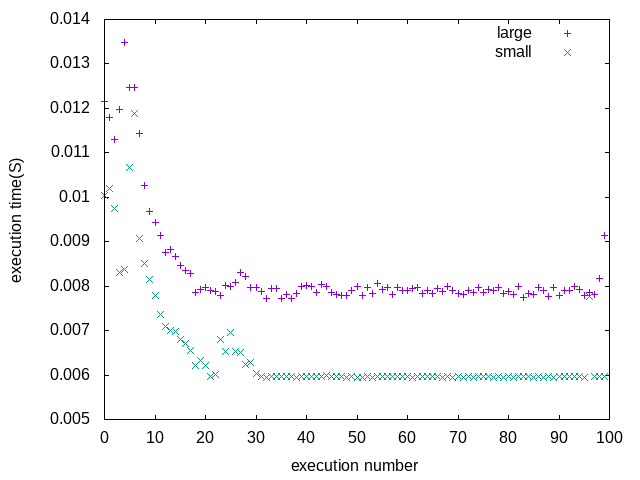
\includegraphics[width=0.8\textwidth]{time.png}
        \caption{Execution time comparison between the small and large headers}
        \label{fig:time}
    \end{figure}

The last graph (see Figure \ref{fig:time}) clearly shows that we get a performance increase in having a smaller memory overhead, at least when the
 test is done where the average allocated block is as small as 16 bytes. At first the tests showed no major difference between 
 using the different block heads, but with some optimization during code compilation the result is what can bee seen in
the graph. This could be that the difference is so insignificant(a time scale of mS) when the code is not optimized, and 
by removing some unnecessary parts of the code the difference shows more clearly. 

The increase in performance probably comes from that the decrease in memory overhead from 24 to 8 per allocated block enables 
a total decrease in the allocated memory area from 40,000 to 24,000 bytes – a decrease in 40 percent. This makes it so that 
it is easier to store the blocks in the computers cache memory for faster access to the processor. The smaller block heads also 
result in a smaller number of bytes needed to be traversed which could contribute 
to the performance increase, but how much this contributes compared to the better use of cache memory these tests do not show.

\newpage

\section{Conclusions}\label{conclusions}

It can be clearly stated that the memory allocating algorithm an operating system uses to allocate and deallocate
 the physical memory space affects the overall performance of a system. An effective algorithm for handling 
 freed memory blocks by merging contiguous free blocks together decreases the memory overhead as well as 
 memory fragmentation - both internal and external.
 
 These improvements will of course come with the cost of more complex algorithms using up resources to accomplish this 
 increase in memory usage. The process of finding the perfect balance in the trade-off between time versus space in computer resource 
 management is something which has been an important part of computer resource management throughout the history of computers and 
 will continue until the day of infinite computing resources - a day wich most likely never will come. 
 
 The algorithms tested in this paper are similar to the ones used by modern OSs of today and the fact that modern computer work 
 with memory sizes in the order of gigabytes instead of kilobytes used in this paper makes it unlikely that the performance increase 
 from scaling down on header sizes will have a huge effect on modern computers overall performance - so those performance test results 
 should not be overstated. But it should still be a goal to minimize memory overhead - just not at all cost.
 The process of merging contigous free blocks however showed to have a big impact in these tests and should show similar behaviour 
 in modern computers, so it is understandable that merging is a standardized practice. Finding even better solutions to the time-space 
 trade off is a continous process and it will be interesting to see what the future has to offer in the world of memory management.

\end{document}

  